\documentclass[titlepage]{article}

\usepackage[hidelinks]{hyperref}
\usepackage[table]{xcolor}
\usepackage[english]{babel}
\usepackage{tabularx}
\usepackage[toc,page]{appendix}
\usepackage{gantt}
\setcounter{secnumdepth}{5}
\usepackage{tikz}
\usepackage{enumitem}
%
\usetikzlibrary{arrows, trees, positioning, fit, calc, shadows.blur, shapes.symbols}

\usepackage[top=1.5in, bottom=1.5in, left=2in, right=2in]{geometry}

\def\getfirstword#1{%
    \begingroup
    \edef\@tempa{#1\space}%
    \expandafter\endgroup
    \expandafter\readwords\@tempa\relax
}
\def\readwords#1 #2\relax{%
      \doword{#1}%  #1 = substr, #2 = rest of string
}
\def\doword#1{#1}
\def\endtestwords{}

\newcommand{\myparagraph}[1]{\paragraph{#1}\mbox{}\\}

\addtolength{\oddsidemargin}{-.875in}
\addtolength{\evensidemargin}{-.875in}
\addtolength{\textwidth}{1.75in}

\def \TACS {Track and Control System}

\begin{document}

\title{
\textbf{
Software Requirements Specification}
\protect\\
for the
\protect\\
\textbf{
Track and Control System}
\protect\\
{\small Version 1.0}}

\author{Robert Moss, Aaron Periera, Matthew Shrago}
\maketitle

%%% Document Approval %%%
\section*{Document Approval}

The following Software Requirements Specification has been accepted and approved by the following:

\begin{center}
    \begin{tabularx}{\textwidth}{ |X|X|X|X| }
    \hline
    \textbf{Signature} & \textbf{Printed Name} & \textbf{Title} & \textbf{Date} \\ \hline
     &  &  &  \\ \hline
     &  &  &  \\ \hline
     &  &  &  \\ \hline
    \end{tabularx}
\end{center}

\newpage
\tableofcontents{} 
\newpage

\section{Introduction}

\subsection{Purpose}
The Software Requirement Specification for the Track and Control System will explain in detail necessary features that the client purposes and the developers provide. The user base will be focused on anyone who will want to use their computer in a more efficient way and take advantage of their full screen space. 

\subsection{Scope}
\begin{enumerate}
	\item Track and Control System
  \begin{enumerate}
  	\item The software will track a user's movements and be able to control numerous features around their Desktop with the movement of their head.
  	\begin{enumerate} 	 	
  		\item The everyday computer user will utilize this software to organize their cluttered Desktop.  	
  	\end{enumerate}
  	\item The application will also act as a security monitor to recognize when you're present at your computer and lock your screen accordingly.
  	\begin{enumerate}
  		\item A benefit of this will be a sense of security for the user when they're away from their computer.
  	\end{enumerate}
  \end{enumerate} 
\end{enumerate}

\subsection{Definitions, Acronyms, and Abbreviations}
\begin{itemize}
	\item Application Specific Definitions
	\begin{itemize}
		\item TACS - Track and Control System
		\item TM - Tracking Module
		\begin{itemize}
			\item OT - Object Tracker
			\item FRT - Facial Recognition Tracker
		\end{itemize}
		\item WCM - Windows Control Module
		\item SM - Settings Module
	\end{itemize}
	\item Industry Definitions
	\begin{itemize}
		\item SRS - Software Requirements Specification
		\item OpenCV - Open Computer Vision: An open source library for object tracking via the camera.
		\item SQLite - A lightweight, low maintenance, self contained local database.
		\item DB - Database
		\item RGB - Red, Green, Blue color values.
		\item HSV - Hue, Saturation, Value.
		\item API - Application Programming Interface
		\item C++ - An object oriented programming language.
		\item GUI - Graphical User Interface
		\item QT - An API for building GUIs
	\end{itemize}
	\item Technical Definitions
	\begin{itemize}
		\item i:j - The range of integers starting at i, increasing to j by 1.
	\end{itemize}
\end{itemize}

\subsection{References}
The list of references below are software documentation that we will be using:
\begin{enumerate}
	\item OpenCV documentation: \href{http://opencv.org/}{\color{blue} http://opencv.org/}
	\begin{itemize}
		\item FaceRecognizer API: \href{http://docs.opencv.org/trunk/modules/contrib/doc/facerec/facerec\_api.html}{\color{blue} http://docs.opencv.org/trunk/modules/contrib/doc/facerec/facerec\_api.html}
	\end{itemize}
	\item Windows API Index: \href{http://msdn.microsoft.com/en-us/library/hh920508(v=vs.85).aspx}{\color{blue} http://msdn.microsoft.com/en-us/library/hh920508(v=vs.85).aspx}
	\item QT C++ documentation: \href{http://qt-project.org/}{\color{blue} http://qt-project.org/}
\end{enumerate}

\subsection{Overview}
The rest of the SRS will contain:
\begin{enumerate}
	\item Specific features of TACS and their details.
	\item System Requirements
	\item Design Constraints for the application.
	\item Risks within the scope.
	\item Any additional information about the development of the application.
\end{enumerate}

\section{General Description}
This section will explicitly lay out the product's functionality and constraints as well as compare it to existing products. Possible set backs will be discussed. Details about each requirement will be in the \nameref{Specific Requirements} section of the SRS. 

\subsection{Product Perspective}
A vast array of other products that utilize OpenCV are available, but no product will control your Desktop with the movement of your head. There has been much research in the field of physical interactions between the user and their computer. However, the application of organizing and securing your Desktop with this interaction is the novel portion of this software.

\subsection{Product Functions}
There will be many available functions the users can utilize. The modular design of the software will allow for additional functions to be easily implemented. \textit{It should be noted that the window functions will be activated with a user-defined hot key.}
\begin{enumerate}
	\item A proportional snap to grid set up for users to place desired windows in five different locations. Namely, left, right, top, bottom, and middle. Once all the windows are selected, the middle window will fill the screen and the user will be able to "peer" in the direction of the four other windows to show a preview of them. 
	\item The software will organize all open windows into a layered view (with the illusion of 3D windows) for the user to "look" around their desktop and see which window they want to select.
	\item The software will be able to detect when the user is away from the screen, and with a user defined delay-time, be able to lock or put your computer to sleep (all settings can be changed from the SM).
\end{enumerate}

\subsection{User Characteristics}
Any computer user who has trouble with screen space will find this software useful. The general user will be a laptop owner who has a built in camera. Anyone from developers to web-surfers with a screen space or battery issue will want to use this software.

\subsection{General Constraints}
\label{General Constraints}
The main functionality of the TM will rely heavily on the availability of an input camera; preferably stationed at the center-top of the screen. If said camera is unavailable, the user can select the mouse as a functional alternative. When using the TM, visibility of the person in control will be crucial.

\subsection{Assumptions and Dependencies}
A camera is assumed to be installed, due to the main functionality incorporating a computer vision tracking module. However, there are alternatives that have been discussed in the \nameref{General Constraints} section.

The windows control module (WCM) is dependent on C++ due to the Windows API written in that language. It is also assumed that the user is running a Windows operating system.

\section{Specific Requirements}
\label{Specific Requirements}
This section will explicitly lay out the purposed system design and it's individual requirements.

\subsection{External Interface Requirements}
\subsubsection{User Interfaces}
A GUI will be built around the two main modules; the TM, and WCM (which both incorporate the SM). It will be written using the open source C++ framework QT 5.2. The GUI will allow the user to change their settings and act as a liaison between each sub-module. Two tabs views for the TM and WCM will give the user a framework for customizing their TACS environment.

\subsubsection{Hardware Interfaces}
An installed camera will send raw data to the TM to be processed. No other external hardware dependencies are necessary.

\subsubsection{Software Interfaces}
The TM will rely on the open source computer vision library, OpenCV 2.4.8, which will be necessary to track the user's movements. For facial recognition, the FRT uses the FaceRecognizer 0.05 API. In addition, the WCM will utilize the easy system calls with the Windows API build date: 3/25/2010.

\subsubsection{Communications Interfaces}
The SM will have direct communication to the local SQLite 3.8.3 database to save user settings. The DB will contain past window configurations of the user, specified delays and hot keys, as well as TM configurations.

\subsection{Functional Requirements}
\subsubsection{Tracking Module (TM)}

\myparagraph{Introduction}
The TM simply tracks the position of the user. Encapsulating it enables the developers to easily swap alternatives for how the user is tracked. A C++ implementation of OpenCV will be used.

\myparagraph{Inputs}
OpenCV will send raw camera data as input to the TM in the form of an $nxm$ matrix that specifies each cell as a pixel with RGB values.

\myparagraph{Processing}
There are several ways in which to process the camera feed. Two main implementations of the TM will be as followed: an object tracker (OT), and a facial recognition tracker (FRT). The OT can apply filters to the matrix of colored pixels coming in as input in a variety of ways. It can filter a specific RGB color in the (0:255, 0:255, 0:255) range and apply a noise reduction algorithm to help pinpoint the target object. The option of HSV filters with the same ranges can yield better results especially in a physical environment that is noisy. The noise tends to increases the uncertainty in the tracked object. The settings for which filter works best in the users physical environment will be sent to the SM to be added to the SQLite DB. The user will have to wear a specific item on their head that can be easily tracked. An alternative to this will be implemented with the FRT.

The FRT, taking advantage of the FaceRecognizer 0.05 API that OpenCV provides, will enable the user to not require any external dependencies for the TM to track. An easy to use API, FaceRecognizer can be a replacement for the OT if the user chooses.  As stated above, all data settings will be saved to the SQLite DB.

If the user does not have a camera, or wished not to have their camera on, they can use the mouse as a suitable replacement for the tracked object. 

\myparagraph{Outputs}
A simple $(x,y)$ coordinate system of the tracked object, whether it be through the OT, FRT, or by mouse, will be given as output of the TM.

\myparagraph{Error Handling}
Uncertainty in the OT will be minimized using filtering algorithms that reduce the tracked object's noise. If the user selects the FRT, then the uncertainty will be lower, due to light restrictions being less harsh, and the specification of the color of your tracked object not necessary. If a clear tracked object isn't present and the mouse tracking isn't enabled, then the system will assume no object and the TM will not output any coordinates.

\subsubsection{Windows Control Module (WCM)}

\myparagraph{Introduction}
The WCM encompasses each real-estate utilizing feature; whether it's space or battery life you're trying to maximize, the WCM will handle everything. All sub-modules will be written in C++ using the Windows API build date: 3/25/2010.

\myparagraph{Inputs}
The outputs of the TM will act as direct inputs to the WCM, namely the $(x,y)$ coordinates of the tracked object. The WCM doesn't care about how the coordinates were calculated, it only worries about manipulating the operating system.

\myparagraph{Processing}
There are three sub-modules to the WCM (with additional features easily added by the developers):
\begin{itemize}
	\item Windows Grid Organizer
	\begin{itemize}[label={}]
		\item The user will be able to select five open windows to be placed in a grid structure around their screen. The top, bottom, left, right, and middle portions will be available for configuration. The user can define the ratio of each window size proportional to the total screen size. This is true for each section except the middle cell; which fills the entire screen once all five windows are chosen. The user can activate the predefined hot-key, defaulted to Alt, and peer in the four outer directions. The middle window will move in the opposite direction to simulate the ``peering'' action of the user. The speed at which the middle cell moves can be altered and saved using the SM.
	\end{itemize}
	\item Windows Perspective (3D)
	\begin{itemize}[label={}]
		\item This feature will organize all open windows into a layered view (with the illusion of 3D windows) for the user to "look" around their desktop and see which window they want to select. The windows in the back layer will move at a much slower rate than the windows in the front layer; to give the illusion of a 3D perspective.
	\end{itemize}
	\item Sleep Manager
	\begin{itemize}[label={}]
		\item If the Sleep Manager is on and the user is away from the computer, the TM will detect that nobody is present and relay that message to the Sleep Manager. The Sleep Manager will then assess if the user is in fact away from the keyboard (via the absence of key presses or mouse movements). If all requirements are aligned, the computer will either lock or sleep after a user defined delay. All of the settings for this configuration will be handled by the SM.
	\end{itemize}
\end{itemize}

\myparagraph{Outputs}
The output of the WCM will be a structure that contains the settings applied to that feature. This structure will be defined in later documents pertaining to design.

\myparagraph{Error Handling}
Each sub-module will have their own set of error handlers. The key component to all of them will be the integrity of the Desktop. 
\begin{itemize}
	\item If the Windows Grid Organizer does not meet all the necessary cells, it will default to empty cells and still be able to function.
	\item The Windows Perspective will have minimal errors associated with it, due in part to the simplistic nature of the feature; only window resizing and repositioning is being applied. 
	\item The Sleep Manager will be handled with care and will default to staying awake with any input from the TM, mouse or keyboard (as to minimize intrusive actions).
\end{itemize}

\subsubsection{Settings Module (SM)}

\myparagraph{Introduction}
The SM will be written in C++ as a transparent module to deal with organizing and saving users data. A local SQLite DB will hold the user's settings for quick access and increased fidelity in TACS.

\myparagraph{Inputs}
The output of the WCM will be a structure of settings for each WCM feature. This structure will be taken in as input to the SM.

\myparagraph{Processing}
The SM, with the predefined structure, will separate the settings by their respective feature. Once separated, the data will be saved to an already created SQLite DB that can be queried at any time.

\myparagraph{Outputs}
A binary variable output will declare if the transaction between the SM and the SQLite DB was successful.

\myparagraph{Error Handling}
If settings were not specified, a list of initial defaults will be available to fall back on.

\subsection{Use Cases}

\subsubsection{Uncooperative/Nonexistent Camera}
\begin{center}
\tikzstyle{arrow}=[draw, -latex]
\begin{tikzpicture} [
	->,
	>=stealth',
	task/.style={
		rectangle,
		draw,
		left color=blue!15,
		right color=black!60!green!60!blue!60,
		rounded corners,
		blur shadow={shadow blur steps=5},
		minimum width=3cm,
		minimum height=1cm
	}
	]
	\node [task] (task2) at (0, 0) {Null Camera Feed?}; 
	\node [task, xshift=5ex,right=of task2] (task3) {Is Camera Available?}; 
	\node [task, xshift=5ex,right=of task3] (task4) at (7, 1.5) {Reinitialize Camera (try once)}; 
	\node [task, xshift=5ex,right=of task4] (task5) at (7, -1.5) {Track Mouse}; 
	
	\path [arrow] (task2) -- node[above] {Yes} ++(task3);
	\path [arrow] (task3) -- node[above] {Yes} ++(task4);
	\path [arrow] (task3) -- node[above] {No} ++(task5);
	\path [arrow] (task4) -| (task2);
\end{tikzpicture}
\end{center}

\subsection{Classes/Objects}
\begin{enumerate}
	\item \textless TrackingModule\textgreater
	\begin{enumerate}
		\item \textless ObjectTracker\textgreater
		\item \textless FacialRecognitionTracker\textgreater
		\item \textless MouseTracker\textgreater
	\end{enumerate}
	\item \textless WindowsControlModule\textgreater
	\begin{enumerate}
		\item \textless WindowsGridOrganizer\textgreater
		\item \textless WindowsPerspective\textgreater
		\item \textless SleepManager\textgreater
	\end{enumerate}
	\item \textless SettingsModule\textgreater
\end{enumerate}

\subsection{Non-Functional Requirements}
\subsubsection{Performance}
The TM should be able to track an object with a 90\% certainty. This can be monitored via an algorithm that takes the users given position, and compares it to the previous one to look for large deviations. If the variance is above a certain threshold, the percentage of certainty will be marked down. A camera feedback of 1 second will be necessary for the TM to talk to the WCM effectively.

\subsubsection{Reliability}
The users customized configuration of their TACS environment will be saved using the SM. This will enable the user to relaunch the program with the same settings as previous sessions.

\subsubsection{Availability}
A internet connection is not necessary for TACS to run, allowing the system to be act independently offline. TACS replies heavily on the installation of a camera, but is not completely dependent on one.

\subsubsection{Security}
The settings that are saved will not require sensitive personal information, so security is a low priority. The use of the camera is the only vulnerability in TACS; however, the lack of internet connectivity means a secure network connection is not necessary. 

\subsubsection{Maintainability}
The modular nature of the design will help developers maintain each encapsulated portion of TACS. Each module can be updated separately, without intruding on it's neighboring modules. Only if there is a redefinition of inputs and outputs will each module need to be updated accordingly.

\subsubsection{Portability}
This software will be built on several machines ranging from Windows 7 (6.1.7601) to Windows 8.1 (6.3.9600). The intended system for use will be a Windows operating system within that range. Because TACS relies heavily on the Windows API, the Linux and Macintosh machine will not be supported.

\subsection{Inverse Requirements}
TACS stresses that the user shouldn't need to learn any proprietary material in order to use the system. Therefore, TACS does not have any inverse requirements.

\subsection{Design Constraints}
Given most laptops come standard will a built-in camera, the design behind TACS is safe. The modular design organizes the individual system features so they can be separately worked on.

\subsection{Logical Database Requirements}
A low maintenance database will be used as a simple data storage facility. This SQLite DB won't need any specific size requirements, due to the minimal amount of data that's required to save.

\section{Project Planning and Risk Management}

% TASK DEFINITIONS: Each task has a given name with newlines (\\) and an alternative name (shortended and without newlines).

\def \Ta {\shortstack{Existing \\ Computer Vision \\ Libraries}}
\def \TaAlt {Research Libraries}

\def \Tb {\shortstack{Learn \\ Dependent \\ APIs}}
\def \TbAlt {Learn API}

\def \Tc {\shortstack{Database \\ Design}}
\def \TcAlt {Database Design}

\def \Td {\shortstack{Software \\ Design}}
\def \TdAlt {Software Design}

\def \Te {\shortstack{Database \\ Development}}
\def \TeAlt {Database Dev.}

\def \Tf {\shortstack{Software \\ Development}}
\def \TfAlt {Software Dev.}

\def \Tg {\shortstack{Analysis \\ and \\ Testing}}
\def \TgAlt {Analysis/Testing}

\def \Th {\shortstack{User \\ Feedback}}
\def \ThAlt {User Feedback}

\def \Y {2014}
\def \Da {1/17}
\def \Db {2/7}
\def \Dc {2/14}
\def \Dd {2/21}
\def \De {3/7}
\def \Df {3/28}
\def \Dg {4/7}
\def \Dh {4/14}

\subsection{Work Breakdown Structure}
\begin{center}
	\begin{tikzpicture}[
	  system/.style={
	  	rectangle,
	  	draw,
	  	top color=blue!0,
	  	bottom color=black!60!green!60!blue!15,
	  	rounded corners=.9ex,
	  	align=center,
	  	node distance=1.5cm,
	  	blur shadow={shadow blur steps=5}
	  },
	  firsttask/.style={
		  rectangle,
		  draw,
		  top color=blue!7,
		  bottom color=black!60!green!60!blue!30,
		  rounded corners=.3ex,
		  align=center,
		  blur shadow={shadow blur steps=5}
	  },
	  secondtask/.style={
		  rectangle,
		  draw,
		  top color=blue!21,
		  bottom color=black!60!green!60!blue!60,
		  text=black,
		  align=center,
		  blur shadow={shadow blur steps=5}
	  },
	  leaftaskshift/.style={
		  grow=down,
		  xshift=-10em
	  },
	  leaftask/.style={grow=down},
	  first/.style={level distance=-2ex},
	  second/.style={level distance=15ex},
	  third/.style={level distance=1ex},
	  fourth/.style={level distance=24ex},
	  level 1/.style={sibling distance=5em}]
	    \coordinate  
	   	% Root
		child[grow=down,first] {node[system]{\TACS}}
		[edge from parent fork down]
			% Children
			child{node[firsttask, xshift=-21ex, yshift=-2ex] {Product Research\\and\\Analysis}
				child[leaftaskshift,second] {node[secondtask,xshift=10ex]{\Ta}}
				child[leaftask,second] {node[secondtask,xshift=6ex]{\Tb}}}
			child{node[firsttask, xshift=-7ex] {Design\\Model}
				child[leaftask,second] {node[secondtask,xshift=-3ex,yshift=3ex]{\Tc}}
				child[leaftask,second] {node[secondtask,xshift=5ex,yshift=-5ex]{\Td}}}
			child {node[firsttask, xshift=7ex] {Application\\Development}
				child[leaftask,second] {node[secondtask,xshift=-3ex,yshift=3ex]{\Te}}
				child[leaftask,second] {node[secondtask,xshift=6ex,yshift=-5ex]{\Tf}}}
			child {node[firsttask, xshift=21ex]{Evaluate\\Application}
				child[leaftask,second] {node[secondtask, xshift=-6ex]{\Tg}}
				child[leaftask,second] {node[secondtask, xshift=6ex]{\Th}}};
	\end{tikzpicture}
\end{center}

\subsection{Time Estimation}

	\begin{center}
	\begin{tikzpicture}
		\node[blur shadow={shadow blur steps=5},fill=white,inner sep=0pt] 
		{\rowcolors{1}{black!40!green!40!blue!40}{black!10!green!10!blue!10}
		\centering
		\begin{tabular}{ |r l| }
		\hline
		\textbf{Task} & \textbf{Weeks} \\
		\hline
		\TaAlt & 1.5 \\
		\TbAlt & 3 \\
		\TcAlt & 1 \\
		\TdAlt & 2 \\
		\TeAlt & 2 \\
		\TfAlt & 5 \\
		\TgAlt & 1 \\
		\ThAlt & 1 \\
		\hline
		\textbf{Total} & \textbf{16.5} \\
		\hline
		\end{tabular}
		};
	\end{tikzpicture}
\end{center}

\subsection{Activity Sequencing Diagram}

\begin{center}
\tikzstyle{arrow}=[draw, -latex]
\begin{tikzpicture} [
	->,
	>=stealth',
	task/.style={
		rectangle,
		draw,
		left color=blue!15,
		right color=black!60!green!60!blue!60,
		rounded corners,
		blur shadow={shadow blur steps=5}
	}
	]
	\node [task, label={[align=center]\Da/\Y}] (task1) at (0, 0) {\Ta}; 
	\node [task, xshift=-3ex, label={[align=center]\Db/\Y},right=of task1] (task2) {\Tb}; 
	\node [task, xshift=3ex, label={[align=center]\Dc/\Y}, minimum width=2cm,right=of task2] (task3) at (3,1) {\Tc}; 
	\node [task, xshift=3ex, label={[align=center,yshift=-10ex]\Dd/\Y}, minimum width=3cm,right=of task3] (task4) at (3,-1) {\Td}; 
	\node [task, xshift=-2ex, yshift=13.5ex, label={[align=center]\De/\Y}, minimum width=2cm, right=of task4] (task5) {\Te}; 
	\node [task, xshift=-0.5ex,  yshift=-13.5ex, xshift=-21ex, label={[align=center,yshift=-10ex]\Df/\Y}, minimum width=3cm,right=of task5] (task6) {\Tf}; 
	\node [task, xshift=-3ex, yshift=13ex, minimum width=3cm, label={[align=center]\Dg/\Y},right=of task6] (task7) {\Tg}; 
	\node [task, xshift=-15ex, yshift=-13ex, minimum width=2cm, label={[align=center,yshift=-10ex]\Dh/\Y},right=of task7] (task8) {\Th}; 
	
	\path [arrow] (task1) -- (task2);
	\path [arrow] (task2) -- (task3);
	\path [arrow] (task2) -- (task4);
	\path [arrow] (task3) -- (task4);
	\path [arrow] (task4) -- (task5);
	\path [arrow] (task4) -- (task6);
	\path [arrow] (task5) -- (task6);
	\path [arrow] (task6) -- (task7);
	\path [arrow] (task7) -- (task8);
\end{tikzpicture}
\end{center}

\subsection{Gantt Chart}
\begin{center}
	\begin{gantt}{9}{12}
		\begin{ganttitle}
	      \titleelement{\Da}{1}
	      \titleelement{\Db}{1}
	      \titleelement{\Dc}{2}
	      \titleelement{\Dd}{1}
	      \titleelement{\De}{2}
	      \titleelement{\Df}{2}
	      \titleelement{\Dg}{2}
	      \titleelement{\Dh}{1}
		\end{ganttitle}
		\ganttbar[color=black!60!green!60!blue!60]{\TaAlt}{0}{1}
		\ganttbar[color=black!60!green!60!blue!60]{\TbAlt}{1}{1}
		\ganttbar[color=black!60!green!60!blue!60]{\TcAlt}{2}{2}
		\ganttbar[color=black!60!green!60!blue!60]{\TdAlt}{2}{3}
		\ganttbar[color=black!60!green!60!blue!60]{\TeAlt}{5}{2}
		\ganttbar[color=black!60!green!60!blue!60]{\TfAlt}{5}{4}
		\ganttbar[color=black!60!green!60!blue!60]{\TgAlt}{9}{2}
		\ganttbar[color=black!60!green!60!blue!60]{\ThAlt}{10}{2}
	\end{gantt}
\end{center}

\subsection{Risk Management}
\begin{table}[h]
	\centering
	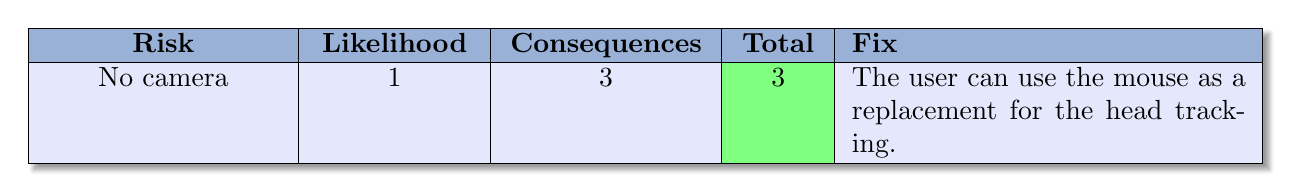
\begin{tikzpicture}
	\node[blur shadow={shadow blur steps=5},fill=white,inner sep=0pt] 
	{\rowcolors{1}{black!40!green!40!blue!40}{black!10!green!10!blue!10}
		\begin{tabular}{ | >{\centering}p{3cm} | >{\centering\arraybackslash}m{2cm} | >{\centering\arraybackslash}m{2.5cm} | >{\centering\arraybackslash}m{1cm} | p{5cm} | }
		\hline
		\textbf{Risk} & \textbf{Likelihood} & \textbf{Consequences} & \textbf{Total} & \textbf{Fix} \\
		\hline
		No camera & 1 & 3 & \cellcolor{green!50}3 & The user can use the mouse as a replacement for the head tracking. \\
		\hline
		\end{tabular}
	};
	\end{tikzpicture}
\end{table}

\newpage
\appendix
\section{Appendix}
\subsection{Design Concept}
A tentative conceptual design of the system is as followed:
\begin{center}
	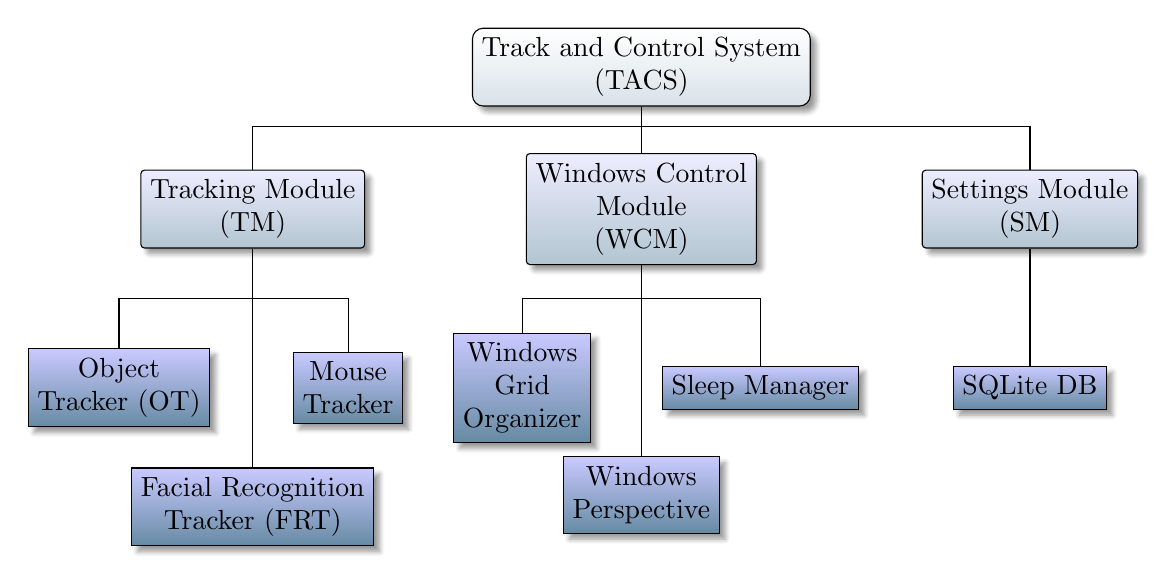
\begin{tikzpicture}[
	  system/.style={
	  	rectangle,
	  	draw,
	  	top color=blue!0,
	  	bottom color=black!60!green!60!blue!15,
	  	rounded corners=.9ex,
	  	align=center,
	  	node distance=1.5cm,
	  	blur shadow={shadow blur steps=5}
	  },
	  firsttask/.style={
		  rectangle,
		  draw,
		  top color=blue!7,
		  bottom color=black!60!green!60!blue!30,
		  rounded corners=.3ex,
		  align=center,
		  blur shadow={shadow blur steps=5}
	  },
	  secondtask/.style={
		  rectangle,
		  draw,
		  top color=blue!21,
		  bottom color=black!60!green!60!blue!60,
		  text=black,
		  align=center,
		  blur shadow={shadow blur steps=5}
	  },
	  leaftaskshift/.style={
		  grow=down,
		  xshift=-10em
	  },
	  leaftask/.style={grow=down},
	  first/.style={level distance=-4ex},
	  second/.style={level distance=15ex},
	  third/.style={level distance=1ex},
	  fourth/.style={level distance=24ex},
	  level 1/.style={sibling distance=5em}]
	    \coordinate  
	   	% Root
		child[grow=down,first] {node[system]{\TACS\\(TACS)}}
		[edge from parent fork down]
			% Children
			child{node[firsttask, xshift=-21ex, yshift=-2ex] {Tracking Module\\(TM)}
				child[leaftaskshift,second] {node[secondtask,xshift=12ex]{Object\\Tracker (OT)}}
				child[leaftask,second] {node[secondtask,yshift=-10ex]{Facial Recognition\\Tracker (FRT)}}
				child[leaftask,second] {node[secondtask,xshift=8ex]{Mouse\\Tracker}}}
			child{node[firsttask,yshift=-2ex] {Windows Control\\Module\\(WCM)}
				child[leaftask,second] {node[secondtask,xshift=-10ex]{Windows\\Grid\\Organizer}}
				child[leaftask,second] {node[secondtask,xshift=0ex, yshift=-9ex]{Windows\\Perspective}}
				child[leaftask,second] {node[secondtask,xshift=10ex]{Sleep Manager}}}
			child {node[firsttask, xshift=21ex, yshift=-2ex] {Settings Module\\(SM)}
				child[leaftask,second] {node[secondtask]{SQLite DB}}};
	\end{tikzpicture}
\end{center}

\end{document}